\documentclass{beamer}
\usetheme{Madrid}
\usepackage{array}
\setbeamertemplate{caption}[numbered]
\title[CST 309 M5]{MANAGEMENT OF SOFTWARE SYSTEMS}
\subtitle{Module 5}
\author{Rijin IK}
\institute[VJEC]{Assistant Professor\\Department of Computer Science and Engineering\\Vimal Jyothi Engineering College\\Chemperi}
\begin{document}
	\begin{frame}
		\titlepage
	\end{frame}
   \begin{frame}{Outline}
   \tableofcontents
   \end{frame}
\section{Software Quality}
\begin{frame}{Software Quality}
\textbf{Software Quality}
\begin{itemize}
	\item Software quality can be defined as: An \textbf{effective software process} applied in a manner that \textbf{creates a useful product }that provides measurable value for those \textbf{who produce it and those who use it}. 
	\item The definition serves to emphasize three main points:
	\begin{itemize}
		\item An \textbf{effective software process} establishes the infrastructure that supports any effort at building a high-quality software product. 
		\item A \textbf{useful product} delivers the content, functions, and features that the end user desires, but as 
		important, it delivers these assets in a reliable, error-free way. 
		\item By adding value for both the \textbf{producer and user }of a software product, high-quality software provides 
		benefits for the software organization and the end-user community. 
	\end{itemize}
	
	\end{itemize}
\end{frame}
\begin{frame}{Software Quality}
	\textbf{Garvin’s Quality Dimensions }
	\begin{itemize}
		\item Performance Quality. 
		\begin{itemize}
			\item Performance refers to a \textbf{product’s primary operating characteristics.}
			\item \textbf{Does the software deliver all content, functions, and features that are specified as part of the requirements }model in a way that provides value to the end user?
		\end{itemize} 
	\item Feature quality. 
	\begin{itemize}
		\item Features are \textbf{additional characteristics that enhance the appeal of the product} or service to the user.
		\item Does the software provide features that surprise and delight first-time end users?
	\end{itemize}
\item Reliability. 
\begin{itemize}
	\item \textbf{Does the software deliver all features and capability without failure?} Is it available when it is needed? Does it deliver functionality that is error free?
\end{itemize}
\item Conformance. 
\begin{itemize}
	\item\textbf{ Does the software conform to local and external software standards} that are relevant to the application?
\end{itemize}
	\end{itemize}
\end{frame}
\begin{frame}{Software Quality}
	\textbf{Garvin’s Quality Dimensions cont.. }
	\begin{itemize}
		\item Durability. 
		\begin{itemize}
			\item \textbf{A measure of product life}
			\item \textbf{Can the software be maintained (changed) or corrected (debugged) without the inadvertent generation of unintended side effects?} Will changes cause the error rate or reliability to degrade with time?
		\end{itemize}
		\item Serviceability. 
	\begin{itemize}
		\item \textbf{Can the software be maintained (changed) or corrected (debugged) in an acceptably short time period?} Can support staff acquire all information they need to make changes or correct defects? 
		
	\end{itemize}
	\item Aesthetics. 
\begin{itemize}
	\item \textbf{Aesthetics refers to the appearance of a product or service}
	\item Does our product have a unique style?
	
\end{itemize}
\item Perception. 
\begin{itemize}
	%\item In some situations, you have a set of prejudices that will influence your perception of quality. 
	\item Meaning that \textbf{a product or service can have high scores} on each of the seven dimensions of quality,\textbf{ but still receive a bad rating from customers as a result of negative perceptions from customers or the public.}
\end{itemize}
	\end{itemize}
\end{frame}

\begin{frame}{Software Quality}
	\textbf{McCall’s software quality factors }
	\begin{figure}
		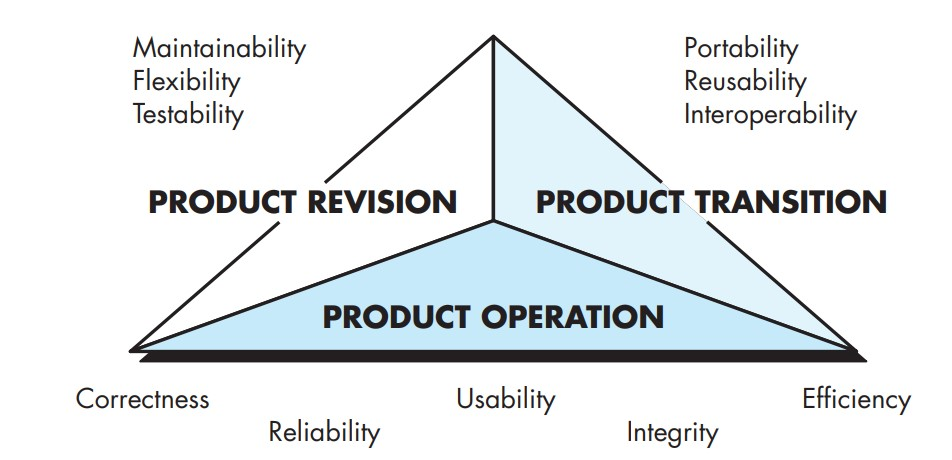
\includegraphics[scale=.3]{img/m5_1}
		\caption{McCall’s 
			software 
			quality factors }
	\end{figure}
	\begin{itemize}
		\item This model classifies all software requirements into 11 software quality factors. 
		\item The 11 factors are grouped into three categories
		\begin{itemize}
			\item \textbf{Product operation factors:} Correctness, Reliability, Efficiency, Integrity, Usability.
			
		\textbf{Product revision factors:}  Maintainability, Flexibility, Testability.
			
		\textbf{Product transition factors:} Portability, Reusability, Interoperability.
		\end{itemize}
	\end{itemize}
\end{frame}
\begin{frame}{Software Quality}
	\textbf{McCall’s software quality factors cont.. }
	\begin{itemize}
			\item \textbf{Correctness:} The extent to which a software meets its requirements specification.
		\item \textbf{Reliability:}The extent to which a software performs its intended functions without failure.
	\item \textbf{Efficiency:} The amount of computing resources and code required by a program to perform its function.
		\item \textbf{Integrity:} Extent to which access to software or data by unauthorized persons can be controlled.
		\item \textbf{Usability:}The extent of effort required to learn, operate and understand the functions of the software.
		\item \textbf{Maintainability:} Effort required to locate and fix an error in a program.
		\item \textbf{Flexibility:} Effort required to modify an operational program.
		\item \textbf{Testability} Effort required to test a program to ensure that it performs its intended function.
	\end{itemize}
\end{frame}

\begin{frame}{Software Quality}
	\textbf{McCall’s software quality factors cont.. }
	\begin{itemize}
		\item \textbf{Portability:} Effort required to transfer the program from one hardware and/or software system environment to another. 
		\item \textbf{Reusability:} Extent to which a program [or parts of a program] can be reused in other applications—related to the packaging and scope of the functions that the program performs.
		\item \textbf{Interoperability:} Effort required to couple one system to another.
	\end{itemize}
\end{frame}
\begin{frame}{Software Quality}
	\textbf{ISO 9216 Quality Factors}
	\begin{itemize}
		\item Functionality.
		\begin{itemize}
			\item  The degree to which the software satisfies stated needs as indicated by the following sub attributes: suitability, accuracy, interoperability, compliance, and security.
		\end{itemize}
		\item Reliability.
		\begin{itemize}
			\item  The amount of time that the software is available for use as indicated by the following sub attributes: maturity, fault tolerance, recoverability.
		\end{itemize}
		\item Usability .
		\begin{itemize}
			\item  The degree to which the software is easy to use as indicated by the following sub attributes: understandability,  learnability, operability.
		\end{itemize}
		\item Efficiency.
		\begin{itemize}
			\item  The degree to which the software makes optimal use of system resources as indicated by the following sub attributes: time behavior, resource behaviour.
		\end{itemize}
	\end{itemize}
\end{frame}
\begin{frame}{Software Quality}
	\textbf{ISO 9216 Quality Factors cont..}
	\begin{itemize}
		\item Maintainability.
		\begin{itemize}
			\item  The ease with which repair may be made to the software as indicated by the following sub attributes: analyzability, changeability, stability, testability.
		\end{itemize}
		\item Portability. 
		\begin{itemize}
			\item The ease with which the software can be transposed from one environment to another as indicated by the following sub attributes: adaptability, installability, conformance, replaceability
		\end{itemize}
		
	\end{itemize}
\end{frame}
\section{Software Quality Dilemma}
\begin{frame}{Software Quality Dilemma}
	\textbf{Software Quality Dilemma cont..}
	\begin{itemize}
		\item The quality dilemma is basically two fold:
		\begin{itemize}
			\item Build bad software (low quality) and no one will want to buy/use it.
			\item Spend too much time on quality measures and no one gets to buy/use it because it either costs too much, or is still being worked on.
		\end{itemize}
		\item Either you missed the market window, or you simply exhausted all your resources.  
		\item So people in industry try to get to that magical middle ground where the product is good enough not to be rejected right away, such as during evaluation, but also not the object of so much perfectionism and so much work that it would take too long or cost too much to complete.
	\end{itemize}
\end{frame}
\begin{frame}{Software Quality Dilemma}
	\textbf{Software Quality Dilemma}
	\begin{itemize}
		\item  \textbf{“Good Enough” Software:}
		\begin{itemize}
			\item Good enough software \textbf{delivers high quality functions and features} that end-users desire,\textbf{ but at the       same time} it delivers other more unclear or specialized functions and features \textbf{that contain known bugs .}
		\end{itemize}
		\item \textbf{The Cost of Quality:}
		\begin{itemize}
			\item  Includes all costs incurred in the pursuit of quality or in performing quality-related activities and the downstream costs of lack of quality.
				\item The cost of quality can be divided 
			into costs associated with prevention, appraisal, and failure.
			\begin{itemize}
				\item \textbf{Prevention:} management activities, training, test planning
				\item \textbf{Appraisal:} technical reviews, data collection and metrics, testing and debugging
				\item \textbf{Failure}\\
			
					 \textbf{Internal:} repair work, network hiccups\\
					\textbf{External:}product return and replacement, help-line
			
			\end{itemize}
		\end{itemize}
	
		\item \textbf{Risks:}
		\begin{itemize}
			\item  The implication is that low-quality software increases risks for both the developer and the end user.
		\end{itemize}
	
	\end{itemize}
\end{frame}
\begin{frame}{Software Quality Dilemma}
	\textbf{Software Quality Dilemma cont..}
	\begin{itemize}
			\item \textbf{Negligence and Liability:}
			\begin{itemize}
				\item  \textbf{Work begins with the best of intentions on both sides}, but \textbf{by the time the system is delivered, things have gone bad}. The system is late, \textbf{fails to deliver desired features and functions}, is error-prone, and \textbf{does not meet with customer approval}. Legal actions happens.
			\end{itemize}
		\item \textbf{Quality and Security:} 
		\begin{itemize}
			\item software that\textbf{ does not exhibit high quality is easier to hack}, and as a consequence, \textbf{low-quality} software can indirectly \textbf{increase the security risk} with all of its attendant costs and problems.
		\end{itemize}
		\item \textbf{The Impact of Management Actions:}
		\begin{itemize}
			\item  Software \textbf{quality is often influenced as much by management decisions} as it is by technology decisions. Even the \textbf{best software engineering practices can be subverted by poor business decisions} and questionable project management actions.
		\end{itemize}
		
	\end{itemize}
\end{frame}
\section{Achieving Software Quality}
\begin{frame}{Achieving Software Quality}
	\textbf{Achieving Software Quality}\\
	Software quality doesn’t just appear. It is the result of good project management and solid software engineering practice, Management and practice are applied within the context of \textbf{four broad activities that 
		help a software team achieve high software quality:}
	
	\begin{itemize}
		\item[1] \textbf{Software Engineering Methods :}
		\begin{itemize}
			\item If you expect to build high-quality software, you must understand the problem to be solved.
			\item You must also be capable of creating a design that conforms to the problem while at the same time exhibiting characteristics that lead to software that exhibits the quality dimensions and factors.
		\end{itemize} 
		\item[2]\textbf{ Project Management Techniques:} Software quality can be improved if 
		\begin{itemize}
			\item[i] a project manager uses estimation to verify that delivery dates are achievable, 
			\item[ii] schedule dependencies are understood and the team resists the temptation to use shortcuts, 
			\item[iii] risk planning is conducted 
		\end{itemize}
	\end{itemize}
\end{frame}
\begin{frame}{Achieving Software Quality con}
	\textbf{Achieving Software Quality cont..}
	\begin{itemize}
		\item[3] \textbf{Quality Control: }
		\begin{itemize}
			\item Quality control encompasses a set of software engineering actions that help to\textbf{ ensure that each work product meets its quality goals.}
			\item A combination of measurement and feedback allows a software team to tune the process when any of these work products fail to meet quality goals.
		\end{itemize} 
		\item[4] \textbf{Quality Assurance: }
		\begin{itemize}
			\item Quality assurance (QA) is any \textbf{systematic process used to determine if a product or service meets quality standards.}
			\item Quality assurance establishes the infrastructure that supports solid software engineering methods, rational project management, and quality control actions—all pivotal if you intend to build high-quality software.
		\end{itemize}
	\end{itemize}
\end{frame}
\begin{frame}{Software Quality Assurance}
	\textbf{Software Quality Assurance}
	\begin{itemize}
		\item Software quality assurance (often called quality management ) is an activity that is applied throughout the software process.
		\item Software quality assurance (SQA) encompasses: 
		\begin{enumerate}
			\item an \textbf{SQA process}, 
			\item specific \textbf{quality assurance and quality control tasks} (including technical reviews and a multi-tiered testing strategy), 
			\item effective \textbf{software engineering practice} (methods and tools), 
			\item control of all software\textbf{ work products and the changes made to them }, 
			\item a \textbf{procedure to ensure compliance with} software development \textbf{standards} (when applicable), and 
			\item \textbf{measurement and reporting mechanisms.}
			
		\end{enumerate}
	\end{itemize}
\end{frame}
\section{Elements of Software Quality Assurance}
\begin{frame}{Elements of Software Quality Assurance}
	\textbf{Elements of Software Quality Assurance}
	\begin{enumerate}
		\item Standards
		\item Reviews and audits
		\item Testing
		\item Error/defect collection and analysis.
		\item Change management.
		\item Education. 
		\item Vendor management
		\item Security management
		\item Safety
		\item Risk management
	\end{enumerate}
\end{frame}
\begin{frame}{Elements of Software Quality Assurance}
	\textbf{Standards}
	\begin{itemize}
		\item The\textbf{ IEEE, ISO,} and other standards organizations have produced a broad array of software engineering standards and related documents. 
		\item Standards may be adopted voluntarily by a software engineering. \item The job of SQA is to\textbf{ ensure that standards that have been adopted are followed and that all work products conform to them.}
	\end{itemize}
	\textbf{Reviews and audits}
\begin{itemize}
	\item Technical reviews are a \textbf{quality control activity} performed by software engineers for their intent is \textbf{to uncover errors.} 
	\item\textbf{Audits} are a\textbf{ type of review} performed by SQA personnel with the intent of \textbf{ensuring that quality guidelines are being followed} for software engineering work.
\end{itemize}
\end{frame}
\begin{frame}{Elements of Software Quality Assurance}
	\textbf{Testing}
	\begin{itemize}
		\item Software testing is a quality control function that has one primary goal – \textbf{to find errors}. The job of SQA is to \textbf{ensure that testing is properly and efficient conducted.}
		
	\end{itemize}
	\textbf{Error/defect collection and analysis}
	\begin{itemize}
		\item SQA \textbf{collects and analyzes error and defect} data to better understand how errors are introduced and \textbf{what software engineering activities are best suited to eliminating them.}
	\end{itemize}
\textbf{Change management}
\begin{itemize}
	\item Change is one of the most disruptive aspects of any software project. If it is not properly managed, change can lead to confusion, and confusion almost always leads to poor quality. \textbf{SQA ensures that adequate change management practices have been instituted.}
\end{itemize}
\end{frame}
\begin{frame}{Elements of Software Quality Assurance}
	\textbf{Education}
	\begin{itemize}
		\item Every software organization wants \textbf{to improve its software engineering practices}. A key contributor to improvement is \textbf{education of software engineers, their managers, and other stakeholders}. \textbf{The SQA organization takes the lead in software process} improvement and is a key proponent and sponsor of educational programs.	
	\end{itemize}
	\textbf{Vendor management}
	\begin{itemize}
		\item Three categories of software are acquired from external software vendors— shrink-wrapped packages (e.g., Microsoft Office), a tailored shell  that provides a basic skeletal structure that is custom tailored to the needs of a purchaser, and contracted software that is custom designed and constructed from specifications provided by the customer organization. 
		\begin{itemize}
			\item \textbf{The job of the SQA organization is to ensure that high-quality software results by suggesting specific quality practices that the vendor should follow (when possible)}, and incorporating quality mandates as part of any contract with an external vendor.
		\end{itemize}
	\end{itemize}
\end{frame}
\begin{frame}{Elements of Software Quality Assurance}
	\textbf{Security management.}
	\begin{itemize}
		\item With the increase in cyber crime and new government regulations regarding privacy, every software organization should institute policies that protect data at all levels, establish firewall protection for WebApps, and ensure that software has not been tampered with internally. \textbf{SQA ensures that appropriate process and technology are used to achieve software security.}
	\end{itemize}
	\textbf{Safety}
	\begin{itemize}
		\item Because software is almost always a pivotal component of human-rated systems (e.g., automotive or aircraft applications), the impact of hidden defects can be catastrophic.\textbf{SQA may be responsible for assessing the impact of software failure and for initiating those steps required to reduce risk.}
	\end{itemize}
\end{frame}
\begin{frame}{Elements of Software Quality Assurance}
	\textbf{Risk management}
	\begin{itemize}
		\item The SQA organization \textbf{ensures that risk management activities are properly conducted and that risk-related contingency plans have been established.}
	\end{itemize}
\end{frame}
\section{SQA Tasks}
\begin{frame}{SQA Tasks}
	\textbf{SQA Tasks}
	\begin{itemize}
		\item The Software Engineering Institute recommends a\textbf{ set of SQA activities that address quality
			assurance planning, oversight, record keeping, analysis, and reporting. }
		\item These activities are
		performed (or facilitated) by an independent SQA group that:

		\begin{itemize}
			\item \textbf{Prepares an SQA plan} for a project.
			\item \textbf{Participates in the development} of the project’s software process description
			\item \textbf{Reviews software engineering activities} to verify compliance with the defined software
			process.
			\item \textbf{Audits designated software work products} to verify compliance with those defined as part of
			the software process.
			\item \textbf{Ensures that deviations in software work} and work products \textbf{are documented and handled
				according to a documented procedure}
			\item \textbf{Records any noncompliance} and \textbf{reports to senior management.}
		\end{itemize}
	\end{itemize}
\end{frame}
\begin{frame}{SQA Tasks}
	\textbf{Prepares an SQA plan for a project}
	\begin{itemize}
		\item The plan is \textbf{developed as part of project planning} and is reviewed by all stakeholders. 
		\item Quality assurance activities performed by the software engineering team and the SQA group are governed by the plan.
		\item The plan identifies
		\begin{itemize}
			\item evaluations to be performed,
			\item  audits and reviews to be conducted,
			\item standards that are applicable to the project,
			\item  procedures for error reporting and tracking, 
			\item work products that are produced by the SQA group,
			\item and feedback that will be provided to the software team.
		\end{itemize} 
		
	\end{itemize}
\end{frame}

\begin{frame}{SQA Tasks}
	\textbf{Participates in the development of the project’s software process description}
	\begin{itemize}
		\item The software team selects a process for the work to be performed.
	
			\item The SQA group reviews
				\begin{itemize}
			\item the process description for compliance with organizational policy, 
			\item internal software standards,
			\item externally imposed standards (e.g., ISO-9001),
			\item and other parts of the software project plan.
		\end{itemize}
	\end{itemize}
\end{frame}

\begin{frame}{SQA Tasks}
	\textbf{Reviews software engineering activities to verify compliance with the defined software process. }
	\begin{itemize}
		\item The SQA group identifies, documents, and tracks deviations from the process and verifies that corrections have been made.	
	\end{itemize}
	\textbf{Audits designated software work products to verify compliance with those defined as part of the software process}
	\begin{itemize}
		\item The SQA group reviews selected work products; identifies, documents, and tracks deviations; verifies that corrections have been made; and periodically reports the results of its work to the project manager.
	\end{itemize}

\end{frame}
\begin{frame}{SQA Tasks}
	\textbf{Ensures that deviations in software work and work products are documented and handled according to a documented procedure}
	\begin{itemize}
		\item Deviations may be encountered in the project plan, process description, applicable standards, or software engineering work products. 
	\end{itemize}
	\textbf{Records any noncompliance and reports to senior management}
	\begin{itemize}
		\item Noncompliance items are tracked until they are resolved.
	\end{itemize}
\end{frame}
\begin{frame}{SQA Tasks}
	\textbf{SQA GOALS }
	\begin{itemize}
		\item Requirement’s quality
		\item Design quality
		\item Code quality
		\item Quality control effectiveness
	\end{itemize}
\end{frame}
\begin{frame}{SQA GOALS}
	\textbf{Requirement’s quality}
	\begin{itemize}
		\item The correctness, completeness, and consistency of the requirements model will have a strong influence on the quality of all work products that follow. SQA must ensure that the software team has properly reviewed the requirements model to achieve a high level of quality.
	\end{itemize}
\textbf{Design quality}
\begin{itemize}
	\item Every element of the design model should be assessed y the software team to ensure that it exhibits high quality and that the design itself conforms to requirements.
\end{itemize}

\end{frame}
\begin{frame}{SQA GOALS}
	\textbf{Code quality}
\begin{itemize}
	\item Source code and related work products must conform to local coding standards and exhibit characteristics that will facilitate maintainability.
\end{itemize}
\textbf{Quality control effectiveness}
\begin{itemize}
	\item A software team should apply limited resources in a way that has the highest likelihood of achieving a high–quality result. SQA analyzes the allocation of resources for reviews and testing to assess whether they are being allocated in the most effective manner.
\end{itemize}
\end{frame}
\begin{frame}{Software 
		measurement and metrics}
	\begin{figure}
	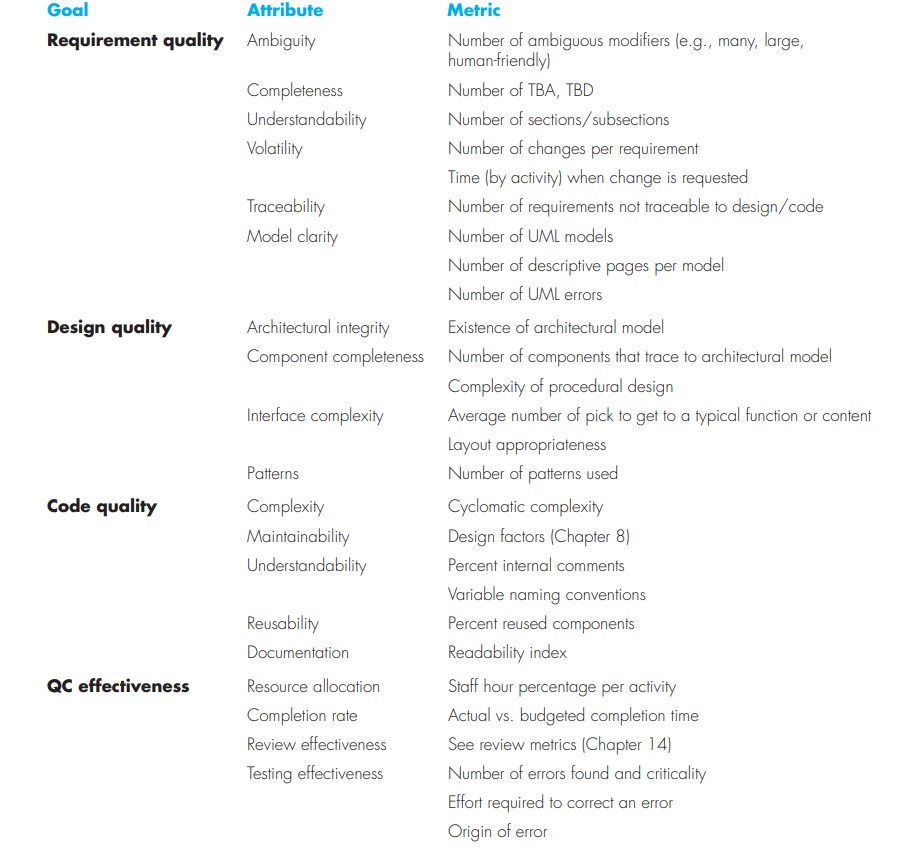
\includegraphics[scale=.4]{img/m5_2}
	\caption{Software quality goals, attributes, and metrics }
\end{figure}
\end{frame}
\section{Software Process Improvement (SPI)}
\begin{frame}{Software Process Improvement (SPI)}
	\textbf{Software Process Improvement (SPI)}
	\begin{itemize}
		\item The term software process\textbf{ improvement (SPI) implies many things. }
		\begin{itemize}
			\item First, it implies that \textbf{elements of an effective software process can be defined in an effective manner; }
			\item second, that an \textbf{existing organizational approach to software development can be assessed against those elements;} 
			\item and third, that \textbf{a meaningful strategy for improvement can be defined. }
		\end{itemize}
	\end{itemize}
The SPI strategy transforms the existing approach to software development into something that is more focused, more repeatable, and more reliable (in terms of the quality of the product produced and the timeliness of delivery).

\end{frame}
\begin{frame}{Software Process Improvement (SPI)}
	\textbf{SPI framework}
	\begin{itemize}
		\item An organization can choose one of the many SPI frameworks.
		\item An SPI framework defines:
		\begin{enumerate}
			\item a \textbf{set of characteristics} that must be present if an effective software process is to be achieved,
			\item a \textbf{method for assessing} whether \textbf{those characteristics are present,}
			\item a \textbf{mechanism for summarizing the results }of any assessment, and 
			\item a \textbf{strategy for assisting a software organization} in implementing those process characteristics that 
			have been found to be weak or missing.

		\end{enumerate}
	\end{itemize}
\end{frame}
\begin{frame}{Software Process Improvement (SPI)}
		\begin{figure}
		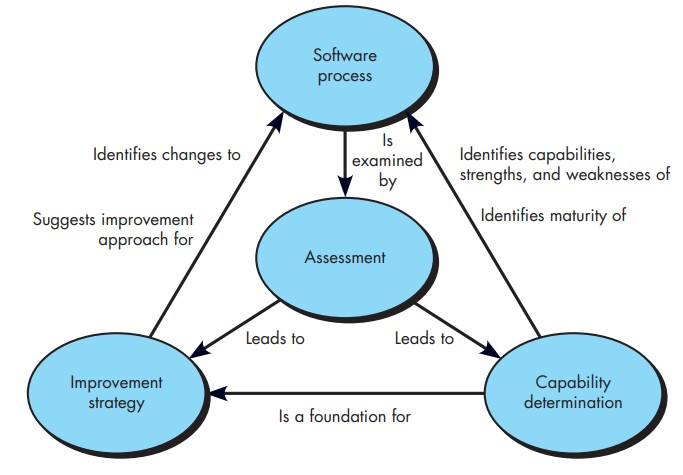
\includegraphics[scale=.4]{img/m5_3}
		\caption{Elements of an SPI framework }
	\end{figure}
\end{frame}
\begin{frame}{Software Process Improvement (SPI)}
\textbf{SPI Process}
\begin{enumerate}
	\item Assessment and Gap Analysis
	\item Education and Training
	\item Selection and Justification
	\item Installation/Migration
	\item Evaluation
	\item Risk Management for SPI
\end{enumerate}
	\end{frame}
\begin{frame}{Software Process Improvement (SPI)}
	\textbf{Assessment and Gap Analysis}
	\begin{itemize}
		\item Assessment examines a wide 
		range of actions and tasks that will lead to a high-quality process.
		\begin{itemize}
			\item \textbf{Consistency.} Are important activities, actions and tasks applied consistently across all software projects and by all software teams?
			\item \textbf{Sophistication.} Are management and technical actions 
			performed with a level of sophistication that implies a 
			thorough understanding of best practice?
			\item\textbf{Acceptance.} Is the software process and software engineering 
			practice widely accepted by management and technical staff?
			\item \textbf{Commitment.} Has management committed the resources 
			required to achieve consistency, sophistication and 
			acceptance?
		\end{itemize}
		
		\item \textbf{Gap analysis}—The difference between local application and 
		best practice represents a “gap” that offers opportunities 
		for improvement.
		
	\end{itemize}
\end{frame}
\begin{frame}{Software Process Improvement (SPI)}
	\textbf{Education and Training}
	\begin{itemize}
		\item It follows that a \textbf{key element of any SPI} strategy \textbf{is education and training} for practitioners, technical 
		managers, and more senior managers who have direct contact with the software organization.
		\item \textbf{Three types 
			of education and training} should be conducted:
		\begin{itemize}
			\item generic software engineering concepts and methods
			\item specific technology and tools
			\item communication and quality-oriented topics.
		\end{itemize} 
	\end{itemize}
\end{frame}
\begin{frame}{Software Process Improvement (SPI)}
	\textbf{Selection and Justification}
	\begin{itemize}
		\item \textbf{Choose the process model that best fits} your organization, its stakeholders, and the software that you build. ?
		\item \textbf{Decide on the set of framework activities }that will be applied, the major work products that will be produced and the quality assurance checkpoints that will enable your team to assess progress. ?
		\item \textbf{Develop a work breakdown for each framework activity} (e.g., modeling), defining the task set that would be applied for a typical project. ?
		\item Once a choice is made, time and money must be expended to install it within an organization and these resource expenditures should be justified.
	\end{itemize}
\end{frame}
\begin{frame}{Software Process Improvement (SPI)}
	\textbf{Installation/Migration}
	\begin{itemize}
		\item \textbf{Installation} is the first point at which a software organization feels \textbf{the effects of changes implemented} as a 
		consequence of the SPI road map. \textbf{In some cases, an entirely new process is recommended for an 
			organization. }
		\item \textbf{In other cases, changes} associated with SPI\textbf{ are relatively minor, representing small, but meaningful 
		modifications to an existing process model}. Such changes are often referred to as\textbf{ process migration}. 
		\item Installation and migration are actually \textbf{software process redesign (SPR)} activities. 
		\item When a formal approach to SPR is initiated, three different 
		process models are considered:
		
		\begin{itemize}
			\item the existing (“as-is”) process, ?
			\item a transitional (“here-to-there”) process,
			\item The target (“to be”) process.
		\end{itemize}
	\end{itemize}
\end{frame}
\begin{frame}{Software Process Improvement (SPI)}
	\textbf{Evaluation}
	\begin{itemize}
		\item \textbf{Assesses the degree to which changes have been instantiated and adopted,} ?
		\item The degree to which such \textbf{changes result in better software quality }or other tangible process benefits.
		\item \textbf{The overall status of the process} and the organizational culture as SPI activities proceed
	\end{itemize}
\end{frame}
\begin{frame}{Software Process Improvement (SPI)}
	\textbf{Risk Management for SPI}
	\begin{itemize}
		\item SPI is a risky undertaking. In fact, more than half of all SPI efforts end in failure. The reasons for failure vary greatly and are organizationally specific. Among the most \textbf{common risks are: }
		\begin{enumerate}
			\item a lack of management support, 
			\item cultural resistance by technical staff, 
			\item a poorly planned SPI strategy, 
			\item an overly formal approach to SPI,
			\item selection of an inappropriate process, 
			\item a lack of buy-in by key stakeholders, 
			\item an inadequate budget, 
			\item a lack of staff training, 
			\item organizational instability, and 
			\item a myriad of other factors. 
		\end{enumerate}
	\item The role of those chartered with the responsibility for SPI is to analyze likely risks and develop an internal strategy for mitigating them.
	\end{itemize}
\end{frame}
\section{CMMI process improvement framework}
\begin{frame}{CMMI process improvement framework}
	\textbf{CMMI process improvement framework}
	\begin{itemize}
		\item \textbf{Capability Maturity Model Integration}
		\item The Capability Maturity Model Integration (CMMI) \textbf{helps organizations} streamline \textbf{process improvement, encouraging a productive, efficient culture that decreases risks} in software, product, and service development.
		\item Each process area (e.g., project planning or requirements management) is formally assessed against specific goals and practices and is \textbf{rated according to the following capability levels:}
		\begin{enumerate}
			\item Level 0: Incomplete 
			\item Level 1: Performed 
			\item Level 2: Managed 
			\item Level 3: Defined 
			\item Level 4: Quantitatively managed
			\item Level 5: Optimized 
		\end{enumerate}
	\end{itemize}
\end{frame}
\begin{frame}{CMMI process improvement framework}
	\textbf{CMMI process improvement framework}
	\begin{itemize}
		\item \textbf{Level 0: Incomplete} 
		\begin{itemize}
			\item incomplete process – partially or not performed.
			\item one or more specific goals of process area are not met.
			\item No generic goals are specified for this level.
			\item this capability level is same as maturity level 1.
		\end{itemize}
	\item \textbf{Level 1: Performed} 
	\begin{itemize}
		\item All of the specific goals of the process area (as defined by the CMMI) have been satisfied. 
		\item Work tasks required to produce 
		defined work products are being conducted. 
		\item Process performance may not be stable.
	\end{itemize}

	\end{itemize}
\end{frame}
\begin{frame}{CMMI process improvement framework}
	\textbf{CMMI process improvement framework}
	\begin{itemize}
		\item \textbf{Level 2: Managed} 
		\begin{itemize}
			\item All capability level 1 criteria have been satisfied.
			\item In addition, all work associated with the process area conforms to an organizationally defined policy;
			\item all people doing the work have access to adequate resources to get the job done;
			\item stakeholders are actively involved in the process area as required; 
			\item all work tasks and work products are “monitored, controlled, and reviewed;
			\item and are evaluated for adherence to the process description” 
		\end{itemize}
		\item \textbf{Level 3: Defined}
		\begin{itemize}
			\item All capability level 2 criteria have been achieved.
			\item a defined process is managed and meets the organization’s set of guidelines and standards.
			\item focus is process standardization.
			
		\end{itemize} 
	\end{itemize}
\end{frame}
\begin{frame}{CMMI process improvement framework}
	\textbf{CMMI process improvement framework}
	\begin{itemize}
		\item \textbf{Level 4: Quantitatively managed } 
		\begin{itemize}
			\item All capability level 3 criteria have been achieved.
			\item In addition, the process area is controlled and improved using measurement and quantitative assessment.
			\item “Quantitative objectives for quality and process performance are established and used as criteria in managing the process”. 
		\end{itemize}
		\item \textbf{Level 5: Optimized }
		\begin{itemize}
			\item All capability level 4 criteria have been achieved.
			\item In addition, the process area is adapted and optimized using quantitative (statistical) means to meet changing customer needs and to continually improve the efficacy of the process area under consideration.
		\end{itemize} 
	\end{itemize}
\end{frame}

\section{ISO 9001:2000 for Software}
\begin{frame}{ISO 9001:2000 for Software}
\textbf{ISO 9001:2000 for Software}
\begin{itemize}
	\item ISO 9001:2000 for Software — a generic\textbf{ standard that applies to any organization} that wants \textbf{to improve} the overall \textbf{quality of} the \textbf{products, systems, or services} that it provides.
	\item Therefore, the \textbf{standard is directly applicable to software organizations and companies}. 
	\item The underlying strategy suggested by ISO 9001:2000 is described in the following manner
	\begin{itemize}
		\item  ISO 9001:2000 \textbf{stresses the importance for an organization to identify, implement, manage and continually improve the effectiveness of the processes that are necessary for the quality management system}, and to manage the interactions of these processes in order to achieve the organization’s objectives.
		\item Process\textbf{ effectiveness and efficiency} can be \textbf{assessed} through \textbf{internal or external review} processes and be evaluated on a maturity scale. 
	\end{itemize}
	
	\item ISO 9001:2008 \textbf{has adopted a “plan-do-check-act” cycle }that is applied to the quality management elements of a software project. 
	
\end{itemize}
	
\end{frame}
\begin{frame}{ISO 9001:2000 for Software}
	\textbf{ISO 9001:2000 for Software cont..}
	\begin{itemize}
		\item Within a software context, \textbf{“plan” establishes the process objectives, activities, and tasks necessary to achieve high-quality software} and resultant customer satisfaction. 
		\item \textbf{“Do” implements the software process} (including both framework and umbrella activities). 
		\item \textbf{“Check” monitors and measures the process} to ensure that all requirements established for quality management have been achieved. 
		\item \textbf{“Act” initiates software process} improvement \textbf{activities that continually work to improve the process. }
		\item TickIt can be used throughout the “plan-do-check-act” cycle to ensure that SPI progress is being made. 
		\item TickIT auditors assess the application of the cycle as a precursor to ISO 9001:2008 certification. 
		\item For a detailed discussion of ISO 9001:2008 and TickIT you should examine [Ant06], [Tri05], or [Sch03].
	\end{itemize}
\end{frame}
\section{Cloud-based Software }
\begin{frame}{Cloud-based Software}
\textbf{Cloud-based Software}
\begin{itemize}
	\item The cloud is a very large number of remote servers that are offered for rent by companies that own these servers.
	\item You can rent as many servers as you need, run your software on these servers, and make them available to your customers.
	\item Your customers can access these servers from their own computers or other networked devices such as a tablet or a TV. 
	\item You may rent a server and install your own software, or you may pay for access to software products that are available on the cloud.
	\item The remote servers are “virtual servers,” which means they are implemented in software rather than hardware.
	\item The cloud servers that you rent can be started up and shut down as demand changes.
	\item Software that runs on the cloud can be scalable, elastic, and resilient.
\end{itemize}
\end{frame}
\begin{frame}{Cloud-based Software}
%	\textbf{Cloud-based Software}
	\begin{itemize}
		\item Software that runs on the cloud can be scalable, elastic, and resilient.
			\begin{figure}
			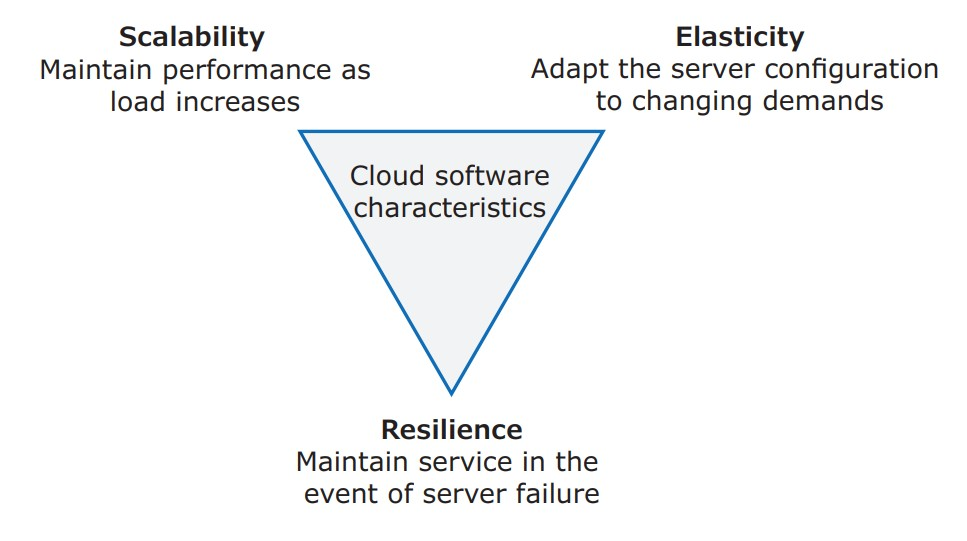
\includegraphics[scale=.4]{img/m5_4}
			\caption{Scalability, elasticity, and resilience}
		\end{figure}
	\end{itemize}
\end{frame}
\begin{frame}{Cloud-based Software}
		\textbf{Benefits of using the cloud for software development}
	
		\begin{figure}
			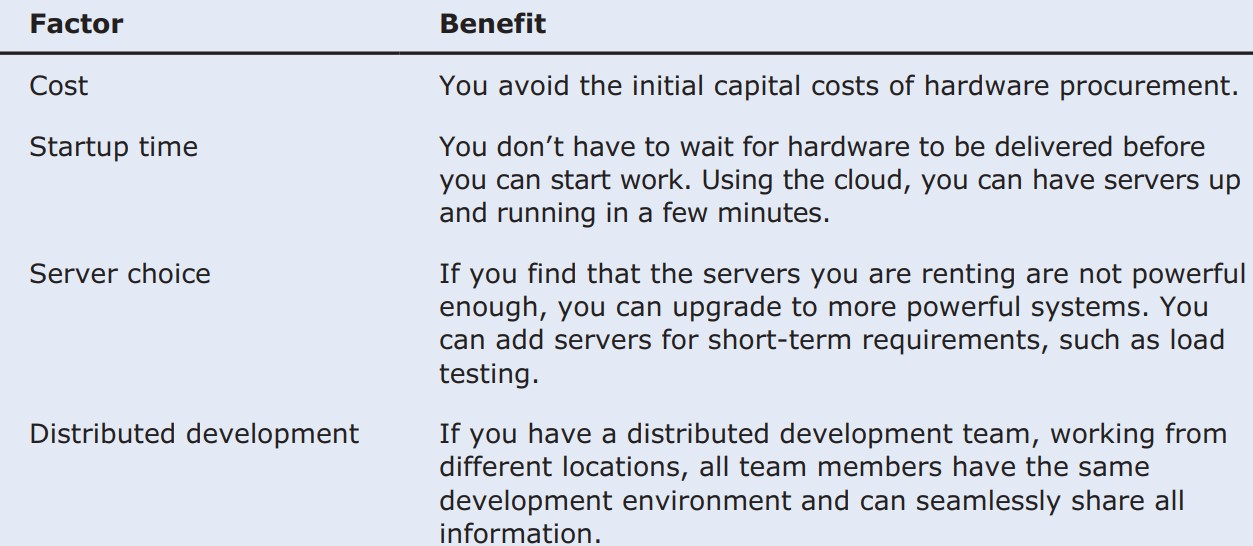
\includegraphics[scale=.4]{img/m5_5}
		%	\caption{Scalability, elasticity, and resilience}
		\end{figure}

\end{frame}
\begin{frame}{Cloud-based Software}
	\textbf{Virtualization and containers}
\begin{itemize}
	\item All cloud servers are\textbf{ virtual servers. }
	\item A virtual server runs on an underlying physical computer and is made up of an operating system plus a set of software packages that provide the server functionality required.
	\item The general idea is that a virtual server is a stand-alone system that can run on any hardware in the cloud.
	\item This “run anywhere” characteristic is possible because the virtual server has no external dependencies. 
\begin{itemize}
		\item An external dependency means you need some software, such as a database management system, that you are not developing yourself.
\end{itemize}
	\item \textbf{Virtual machines (VMs)}, running on physical server hardware, can be used to implement virtual servers.

\end{itemize}	
\end{frame}
\begin{frame}{Cloud-based Software}
	\textbf{Virtualization and containers cont..}
\begin{itemize}
	\item \textbf{Hypervisor}
	\item \textbf{Container }
\end{itemize}
 \textbf{Hypervisor}
	\begin{itemize}
		\item Also known as a\textbf{ virtual machine monitor or VMM,} is software that creates and runs virtual machines (VMs). 
		\item Hypervisor \textbf{providing a hardware emulation} that simulates 
		the operation of the underlying hardware. 
		\item  A hypervisor allows \textbf{one host computer to support multiple guest} VMs by virtually sharing its resources, such as memory and processing.
		\item Several of these hardware emulators share the physical hardware and run in parallel. 
		\item You can run an operating system and then install server software on each hardware emulator.
	\end{itemize}	
\end{frame}
\begin{frame}{Cloud-based Software}
\begin{figure}
	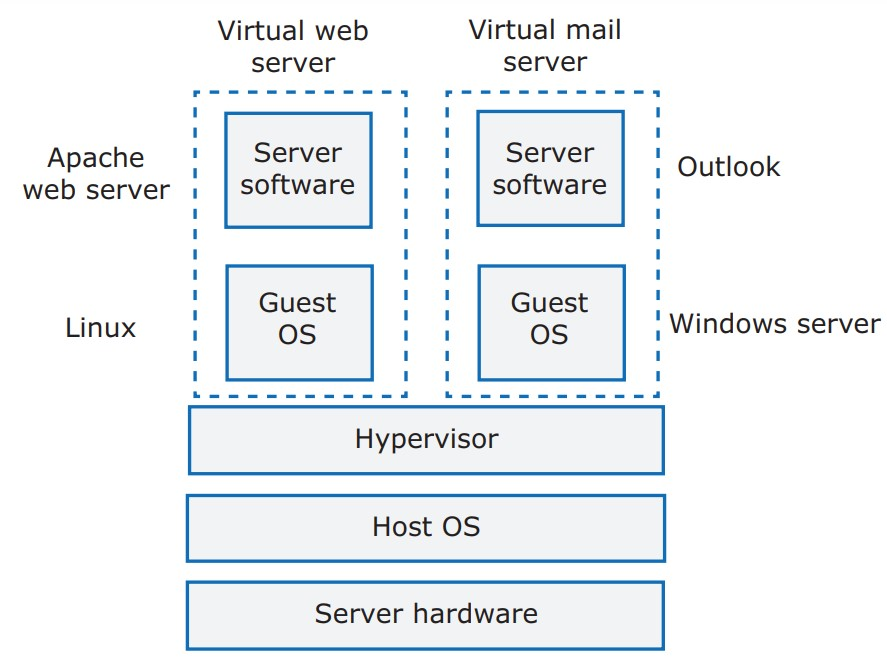
\includegraphics[scale=.4]{img/m5_6}
		\caption{Implementing a virtual server as a virtual machine}
\end{figure}
\end{frame}
\begin{frame}{Cloud-based Software}
	\textbf{Container}
	\begin{itemize}
		\item Containers are an operating system virtualization technology that allows 
		independent servers to share a single operating system.
			\end{itemize}	
	\begin{figure}
		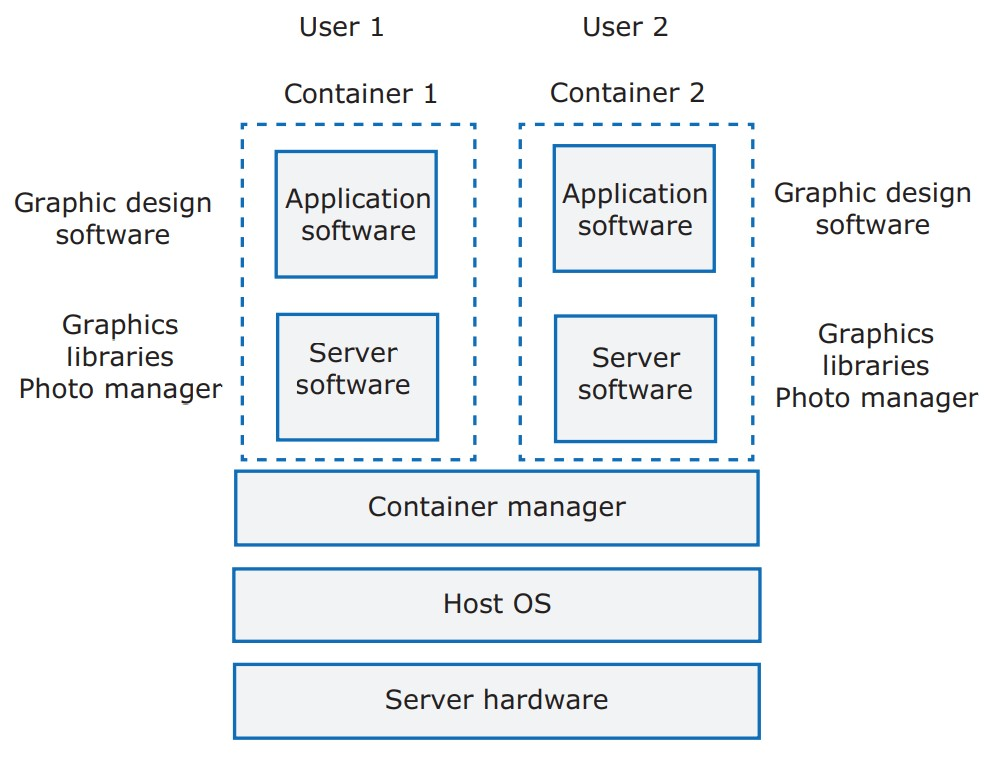
\includegraphics[scale=.35]{img/m5_7}
		\caption{Using containers to provide isolated services}
	\end{figure}
\end{frame}
\begin{frame}{Cloud-based Software}
\textbf{Advantage of using a virtual machine}
	\begin{itemize}
		\item The advantage of using a virtual machine to implement virtual servers is that you have exactly the same hardware platform as a physical server. 
		\item Therefore run different operating systems on virtual machines that are hosted on the same computer
	\end{itemize}		
	
\end{frame}
\begin{frame}{Cloud-based Software}
	\textbf{Everything as a service}
	\begin{figure}
	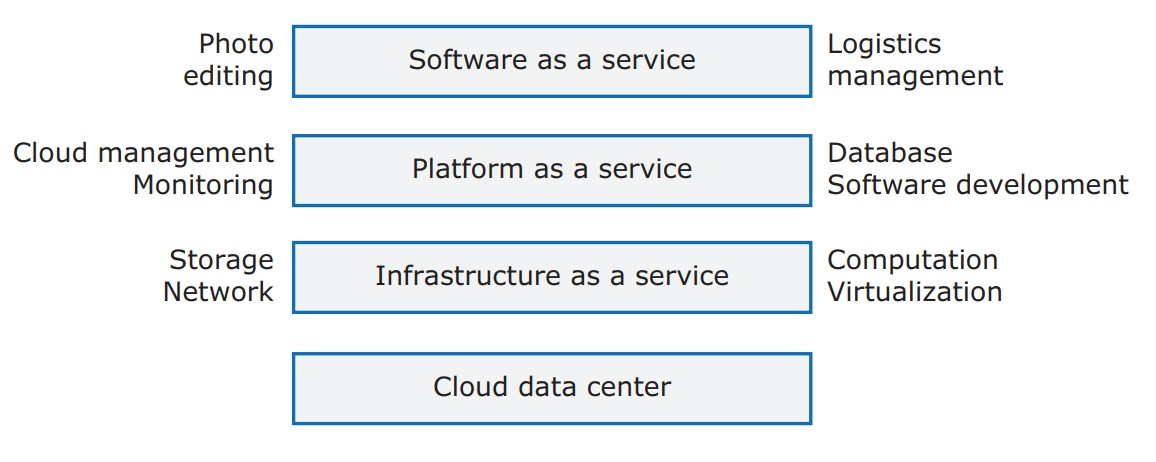
\includegraphics[scale=.5]{img/m5_8}
	\caption{Everything as a service}
\end{figure}
\end{frame}
\begin{frame}{Cloud-based Software}
	\textbf{Infrastructure as a service (IaaS) }
\begin{itemize}
	\item This is a basic service level that all major cloud providers offer. 
	\item IaaS provider provides the following services
	\begin{itemize}
		\item\textbf{Compute:} Computing as a Service includes virtual central processing units and virtual main memory for the Vms that is provisioned to the end- users.
		\item\textbf{Storage:} IaaS provider provides back-end storage for storing files.
		\item\textbf{Network:} Network as a Service (NaaS) provides networking components such as routers, switches, and bridges for the Vms.
		\item\textbf{Load balancers:} It provides load balancing capability at the infrastructure layer.
	\end{itemize}
%\item These infrastructure services may be used to implement virtual cloud-based servers. 
\item The key benefits of using IaaS are
\begin{itemize}
	\item you don’t incur the capital costs of buying hardware and 
	\item you can easily migrate your software from one server to a more powerful server. 
	\item You are responsible for installing the software on the server, although many preconfigured packages 
	are available to help with this. 
	\item Using the cloud provider’s control panel, you can easily add more servers if you need to as the load on your system increases.
\end{itemize}  
\end{itemize}
\end{frame}
\begin{frame}{Cloud-based Software}
	\textbf{Platform as a service (PaaS) }
	\begin{itemize}
		\item This is an intermediate level where you use libraries and frameworks provided by the cloud provider to 
		implement your software.
		\item These provide access to a range of functions, including SQL and NoSQL databases. 
		\item Using PaaS makes it easy to develop auto-scaling software. 
		\item You can implement your product so that as the load increases, additional compute and storage 
		resources are added automatically.
		\item Eg: facebook, Google App Engine, Google Colab, platforms for the data science.
	\end{itemize}
\end{frame}
\begin{frame}{Cloud-based Software}
	\textbf{Software as a service (SaaS) }
	\begin{itemize}
		\item SaaS is also known as "On-Demand Software".
		\item It is a software distribution model in which services are hosted by a cloud service provider. 
		\item These services are available to end-users over the internet so, the end-users do not need to install any software on their devices to access these services.
		\item Your software product runs on the cloud and is accessed by users through a web browser or mobile app.
		\item We all know and use this type of cloud service—mail services such as Gmail, storage services such as Dropbox, social media services such as Twitter, and so on. 
	\end{itemize}
\end{frame}
\begin{frame}{Cloud-based Software}
	\begin{figure}
	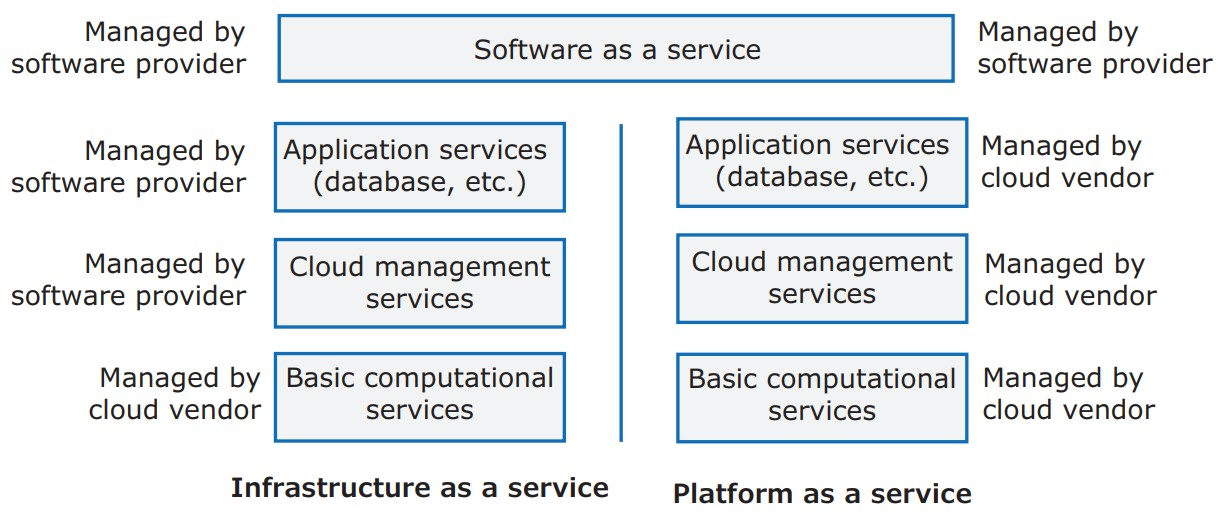
\includegraphics[scale=.4]{img/m5_9}
	\caption{Management responsibilities for SaaS, IaaS, and PaaS}
\end{figure}
\end{frame}
\section{Microservices Architecture}
\begin{frame}{Microservices}
\textbf{Microservices}
\begin{itemize}
	\item Microservices are small-scale, stateless services that have a single responsibility.
	\item Software products that use microservices are said to have a microservices architecture.
	\item If you need to create cloud-based software products that are adaptable, scalable, and resilient, then it is recommend to use a microservices architecture.
\end{itemize}
\end{frame}
\begin{frame}{Microservices}
\begin{itemize}
	\item 	\textbf{Example of Microservices}
		\begin{itemize}
		\item Consider a system that uses an authentication module that provides the following features:
		\begin{itemize}
			\item user registration, where users provide information about their identity, security information, mobile number, and email address;
			\item authentication using user ID (UID)/password;
			\item two-factor authentication using code sent to mobile phone;
			\item user information management—for example, ability to change password or mobile phone number;
			\item password reset.
			
		\end{itemize}
		\item In principle, each of these features can be implemented as a separate service that uses a central shared database to hold authentication information. 
		\begin{itemize}
			\item A user interface service can then manage all aspects of user communication.
			\item In a microservices architecture, however, these features are too large to be microservices. 
			\item To identify the microservices that might be used in the authentication system, you need to break down the coarse-grain features into more detailed functions.
		\end{itemize}
	\end{itemize}
\end{itemize}
\end{frame}
\begin{frame}{Microservices}
	Figure shows what these functions might be for 
	user registration and UID/password authentication.
	\begin{figure}
	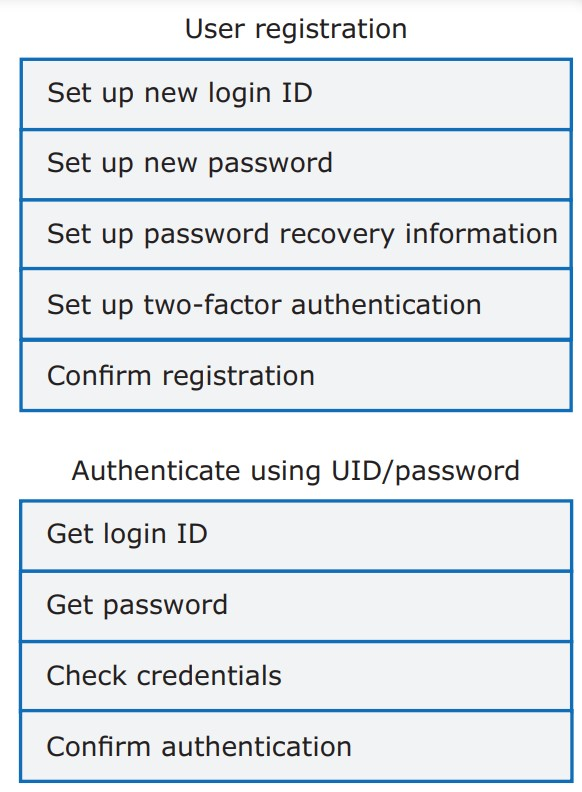
\includegraphics[scale=.3]{img/m5_10}
	\caption{Functional breakdown of authentication features}
\end{figure}
\end{frame}
\begin{frame}{Microservices}
Figure shows the microservices that could be used to 
implement user authentication.
	\begin{figure}
		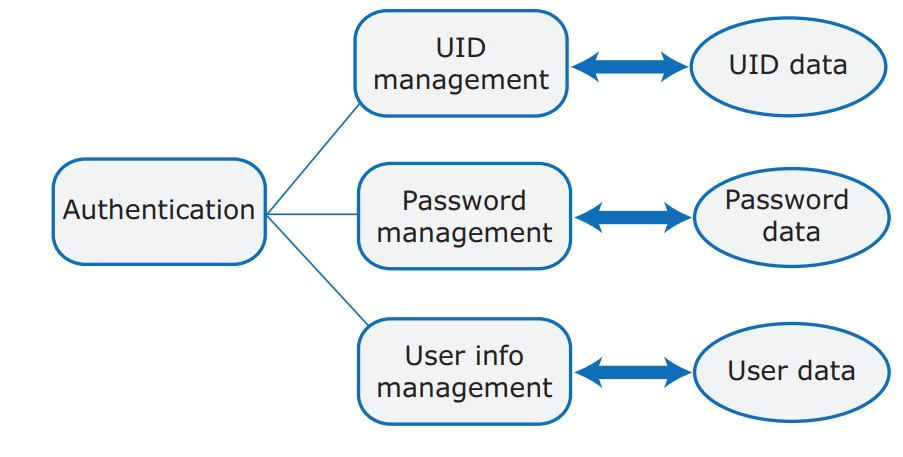
\includegraphics[scale=.3]{img/m5_11}
		\caption{Authentication microservices}
	\end{figure}
\end{frame}
\begin{frame}{Microservices}
	\textbf{Characteristics of microservices}
	\begin{itemize}
		\item \textbf{Self-contained:}Microservices do not have external dependencies. They 
		manage their own data and implement their own user 
		interface.
		\item \textbf{Lightweight:}Microservices communicate using lightweight protocols, 
		so that service communication overheads are low.
		\item \textbf{Implementation-independent:}Microservices may be implemented using different 
		programming languages and may use different 
		technologies (e.g., different types of database) in their 
		implementation.
		\item \textbf{Independently deployable:}Each microservice runs in its own process and is 
		independently deployable, using automated systems.
		\item \textbf{Business-oriented:}Microservices should implement business capabilities and 
		needs, rather than simply provide a technical service.		
	\end{itemize}
\end{frame}

\begin{frame}{Microservices}
	\textbf{Microservice communication}
	\begin{itemize}
		\item Microservices communicate by exchanging messages.	
	    \item A message that is sent between services includes some administrative
		information, a service request and the data required to deliver the
		requested service.
		\item Services return a response to service request messages.
		\begin{itemize}
			\item An authentication service may send a message to a login service that includes
			the name input by the user.
			\item The response may be a token associated with a valid user name or might be an
			error saying that there is no registered user.
		\end{itemize}
	\end{itemize}
\end{frame}
\begin{frame}{Microservices architecture}
	\textbf{Microservices architecture}
	\begin{itemize}
		\item A microservices architecture is a tried and tested way of implementing a logical software architecture.
		\item This architectural style aims to address two fundamental problem with monolithic architecture
		\begin{enumerate}
			\item The whole system has to be rebuilt, re-tested and re-deployed when any
			change is made. This can be a slow process as changes to one part of the
			system can adversely affect other components.
			\item As the demand on the system increases, the whole system has to be scaled,
			even if the demand is localized to a small number of system components that
			implement the most popular system functions.
		\end{enumerate}
	\end{itemize}
\end{frame}
\begin{frame}{Microservices architecture}
	\textbf{Benefits of microservices architecture}
	\begin{itemize}
		\item Microservices are self-contained and run in separate processes.
		\item In cloud-based systems, each microservice may be deployed in its own
		container. This means a microservice can be stopped and restarted
		without affecting other parts of the system.
		\item If the demand on a service increases, service replicas can be quickly
		created and deployed. These do not require a more powerful server so
		‘scaling-out’ is, typically, much cheaper than ’scaling up’.
	\end{itemize}
\end{frame}
\begin{frame}{Microservices architecture}
	\textbf{A microservices architecture for a photo-printing system}
	\begin{itemize}
		\item Imagine that you are developing a photo printing service for mobile devices.
		Users can upload photos to your server from their phone or specify photos from
		their Instagram account that they would like to be printed. Prints can be made at
		different sizes and on different media.
		\item Users can chose print size and print medium. For example, they may decide to
		print a picture onto a mug or a T-shirt. The prints or other media are prepared and
		then posted to their home. They pay for prints either using a payment service
		such as Android or Apple Pay or by registering a credit card with the printing
		service provider.
	\end{itemize}
\end{frame}
\begin{frame}{Microservices architecture}
		\begin{figure}
		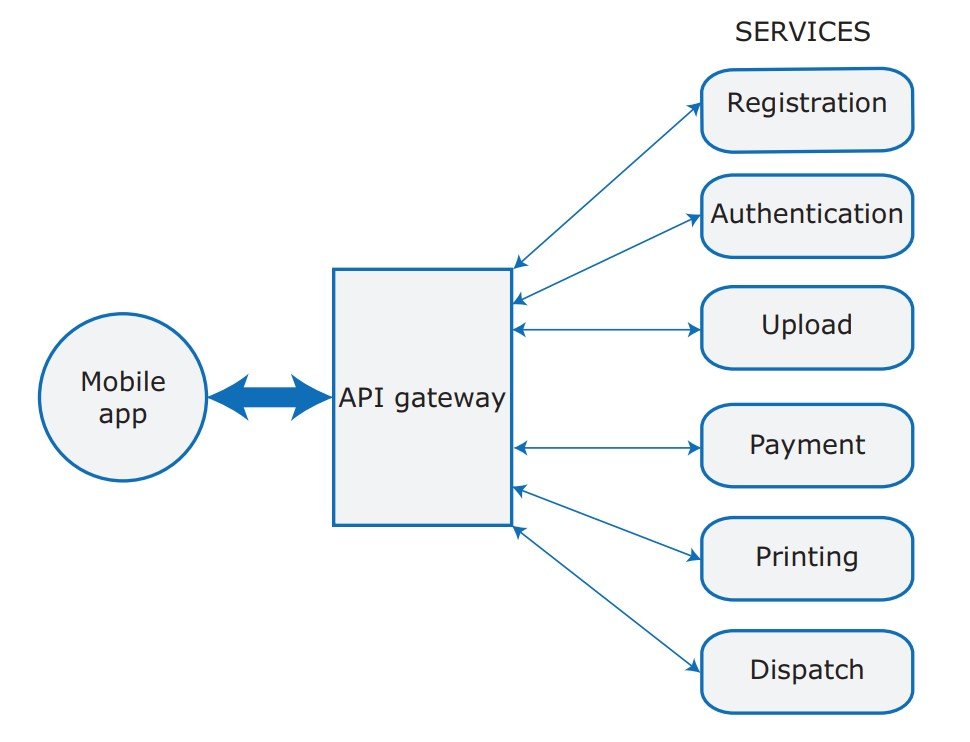
\includegraphics[scale=.3]{img/m5_12}
		\caption{A microservices architecture for a photo-printing system}
	\end{figure}
\end{frame}
\begin{frame}{Microservices architecture}
	\textbf{Architecture Design Decisions}
	\begin{itemize}
		\item In a microservice-based system, the development teams for each service are autonomous.
		\item They make their own decisions about how best to provide the service.
		\item This means the system architect should not 
		make technology decisions for individual services; these are left to the service implementation team. 
	\end{itemize}
\end{frame}
\begin{frame}{Microservices architecture}
	\textbf{Key design questions for microservices architecture}
		\begin{figure}
		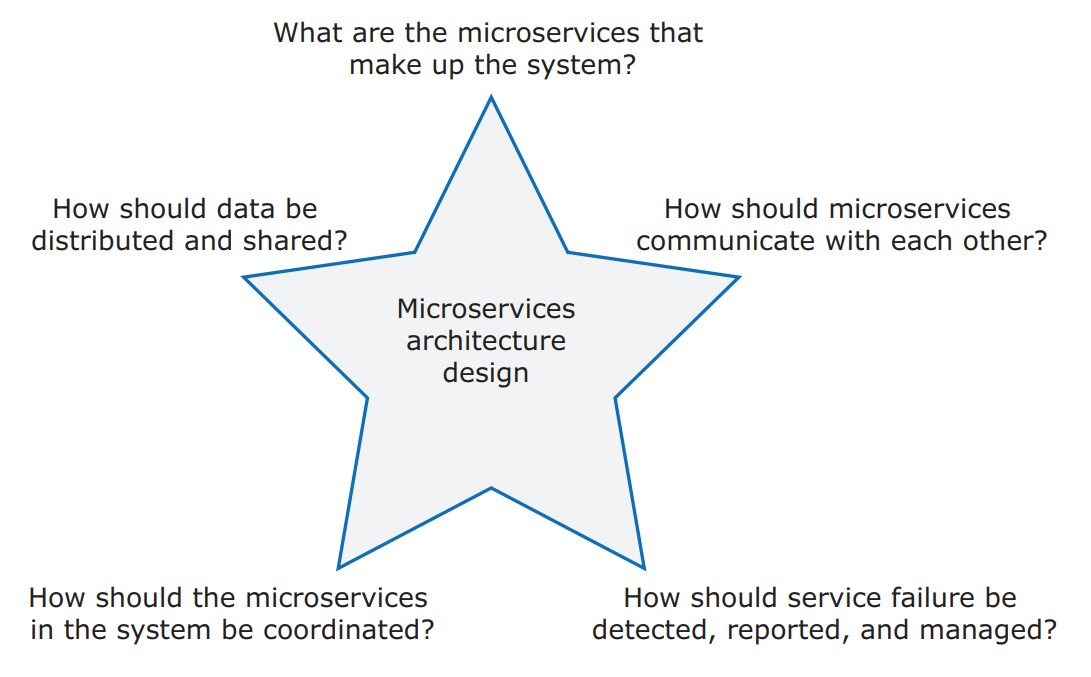
\includegraphics[scale=.3]{img/m5_13}
		\caption{Key design questions for microservices architecture}
	\end{figure}
\end{frame}
\begin{frame}{Microservices architecture}
	\textbf{General Guidelines to decompose microservices}
\begin{itemize}
	\item Balance fine-grain functionality and system performance
	\item Follow the “common closure principle”
	\item Associate services with business capabilities
	\item Design services so that they have access to only the data that they need
\end{itemize}
\textbf{Service Communications}
\begin{itemize}
	\item Services communicate by exchanging messages.
	\item These messages include information about the originator 
	of the message as well as the data that are the input to or output from the request.
	\item Key decisions that you have to make are:
	\begin{itemize}
		\item Should service interaction be synchronous or asynchronous?
		\item Should services communicate directly or via message broker middleware?
		\item What protocol should be used for messages exchanged between services?
	\end{itemize}
\end{itemize}
\end{frame}
\begin{frame}{Microservices architecture}
	\textbf{Data Distributions and Sharing}
	\begin{itemize}
		\item A general rule of microservice development is that each microservice should manage its own data. 
		\item You 
		need to think about the microservices as an interacting system rather than as individual units. This means:
		\begin{itemize}
			\item You should isolate data within each system service with as little data sharing as possible.
			\item If data sharing is unavoidable, you should design microservices so that most sharing is read-only, with 
			a minimal number of services responsible for data updates.
			\item If services are replicated in your system, you must include a mechanism that can keep the database 
			copies used by replica services consistent.
		\end{itemize}
	\end{itemize}
\end{frame}
\begin{frame}{Microservices architecture}
	\textbf{Data Distributions and Sharing}
	\begin{itemize}
		\item Most user sessions involve a series of interactions in which operations have to be carried out in a 
		specific order. This is called a workflow. 
		\item An alternative approach that is often recommended for microservices is called “choreography.”
		\begin{itemize}
			\item This 
			term is derived from dance rather than music, where there is no “conductor” for the dancers.
			\item Rather, 
			the dance proceeds as dancers observe one another. Their decision to move on to the next part of the 
			dance depends on what the other dancers are doing.
		\end{itemize}  
	\end{itemize}
\end{frame}
\begin{frame}{Microservices architecture}
	\textbf{Failure management}
	\begin{itemize}
		\item Three types of failures occur in microservice systems
	\end{itemize}
	\begin{figure}
	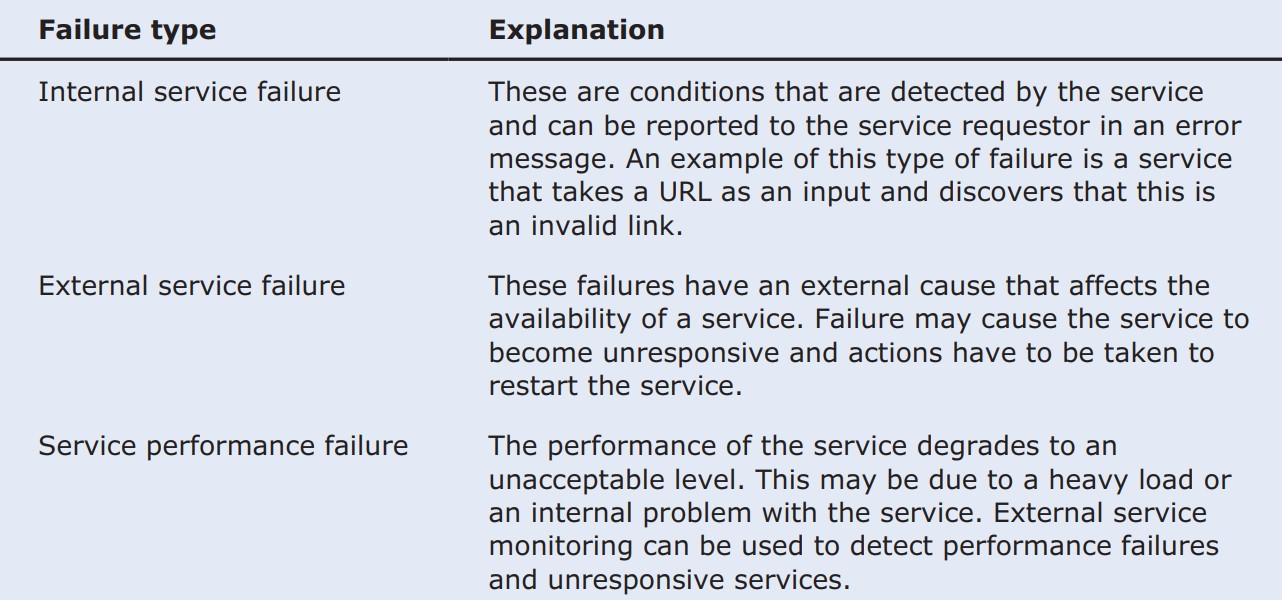
\includegraphics[scale=.35]{img/m5_14}
	\caption{Failure types in a microservices system}
	The simplest way to report microservice failures is to use HTTP status codes, which indicate whether or 
	not a request has succeeded.
\end{figure}
\end{frame}
\begin{frame}{Microservice deployment}
	\textbf{Microservice deployment}
	\begin{itemize}
		\item After a system has been developed and delivered, it has to be deployed on servers, monitored for problems, and updated as new versions become available. 
		\item Traditionally, the tasks of managing an operational system were seen as separate from development. 
		\item The system admin team had different skills from the system developers. 
		\item When a system is composed of tens or even hundreds of microservices, deployment of the system is more complex than for monolithic systems.
	\end{itemize}
\end{frame}
\begin{frame}{Microservice deployment}
	\textbf{Microservice deployment}
	\begin{itemize}
		\item The service development teams decide which programming language, database, libraries, and other support software should be used to implement their service. 
		\item Consequently, there is no “standard” deployment configuration for all services. 
		\item Furthermore, services may change very quickly and there is the potential for a “deployment bottleneck” if a separate system admin team is faced with the problem of updating several services at the same time.
		
	\end{itemize}
\end{frame}
\begin{frame}{Microservice deployment}

	\begin{figure}
		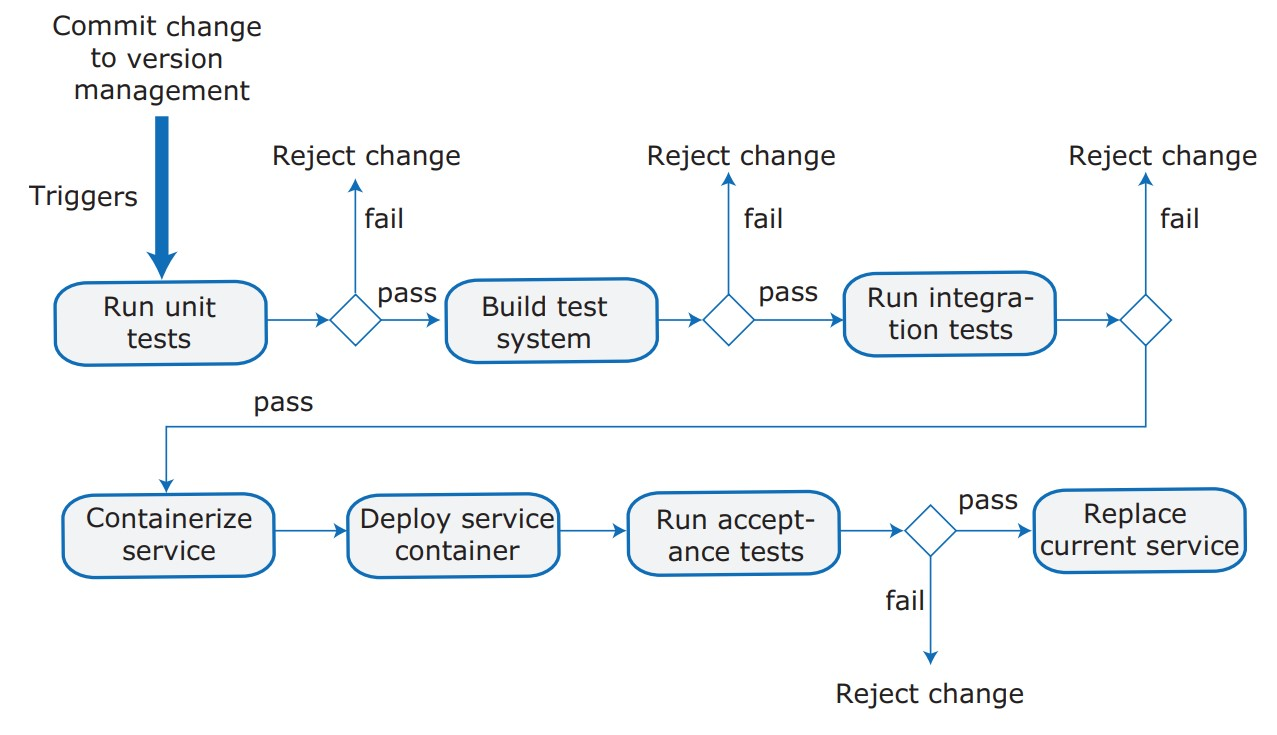
\includegraphics[scale=.3]{img/m5_15}
		\caption{A continuous deployment pipeline}
	\end{figure}
\end{frame}
\end{document}